\chapter[\hspace{0pt}相关研究技术与理论]{{\heiti\zihao{3}\hspace{0pt}相关研究技术与理论}}

\removelofgap
\removelotgap

本章内容共分为五节,\hyperref[section2: 少样本分类]{第一节}详细介绍少样本分类任务;\hyperref[section2: 对比学习]{第二节}介绍与第三章方法相关的对比学习工作;\hyperref[section2: 语义信息表示]{第三节}介绍第四章方法应用到的语义信息表示及一些用来获得语义信息的自然语言处理模型和多模态模型;\hyperref[section2: 数据集及评价指标]{第四节}对本文所使用的数据集和评价指标进行介绍,\hyperref[section2: 本章小结]{第五节}对本章进行小结。

\section[\hspace{-2pt}少样本分类]{{\heiti\zihao{-3} \hspace{-8pt}少样本分类}}\label{section2: 少样本分类}

少样本分类,旨在模拟人类识别新类别的过程,希望模型在拥有大规模标注数据的类别上进行训练之后,能够总结并迁移所学知识到新的类别,以实现在新类别上仅用少量标注数据进行训练便能够达到良好效果的目的。与常规分类任务将数据集划分为训练集与测试集不同,少样本分类数据集被划分为基类数据和新类数据,两者类别互不相交。其中,基类数据与普通分类任务的训练集一致,所有数据均可以被用来训练模型,无论是以元学习还是以普通分类任务的训练方式。而新类数据则是用来测试模型性能,在少样本分类的测试过程中,会在新类数据集上随机采样大量分类任务,每个任务的数据又被划分为支持集与查询集,如图\ref{figure2: 少样本分类测试任务}所示。其中,支持集数据为带有标注的样本,可用来微调整个模型和重新训练分类器,而查询集作用则是类似普通分类任务中的测试集,用来评估模型准确率。根据采样任务中类别数目\emph{N}和样本数目\emph{K}的多少,其又可被称为\emph{N}-way \emph{K}-shot任务,\emph{N}通常取5,\emph{K}通常取1或5。最终,通过对大量采样任务分别进行评估,并计算这些任务的平均准确率作为模型性能的最终评价指标。

\begin{figure}[h!]
\centering
\captionsetup{font={small, stretch=1.312}}
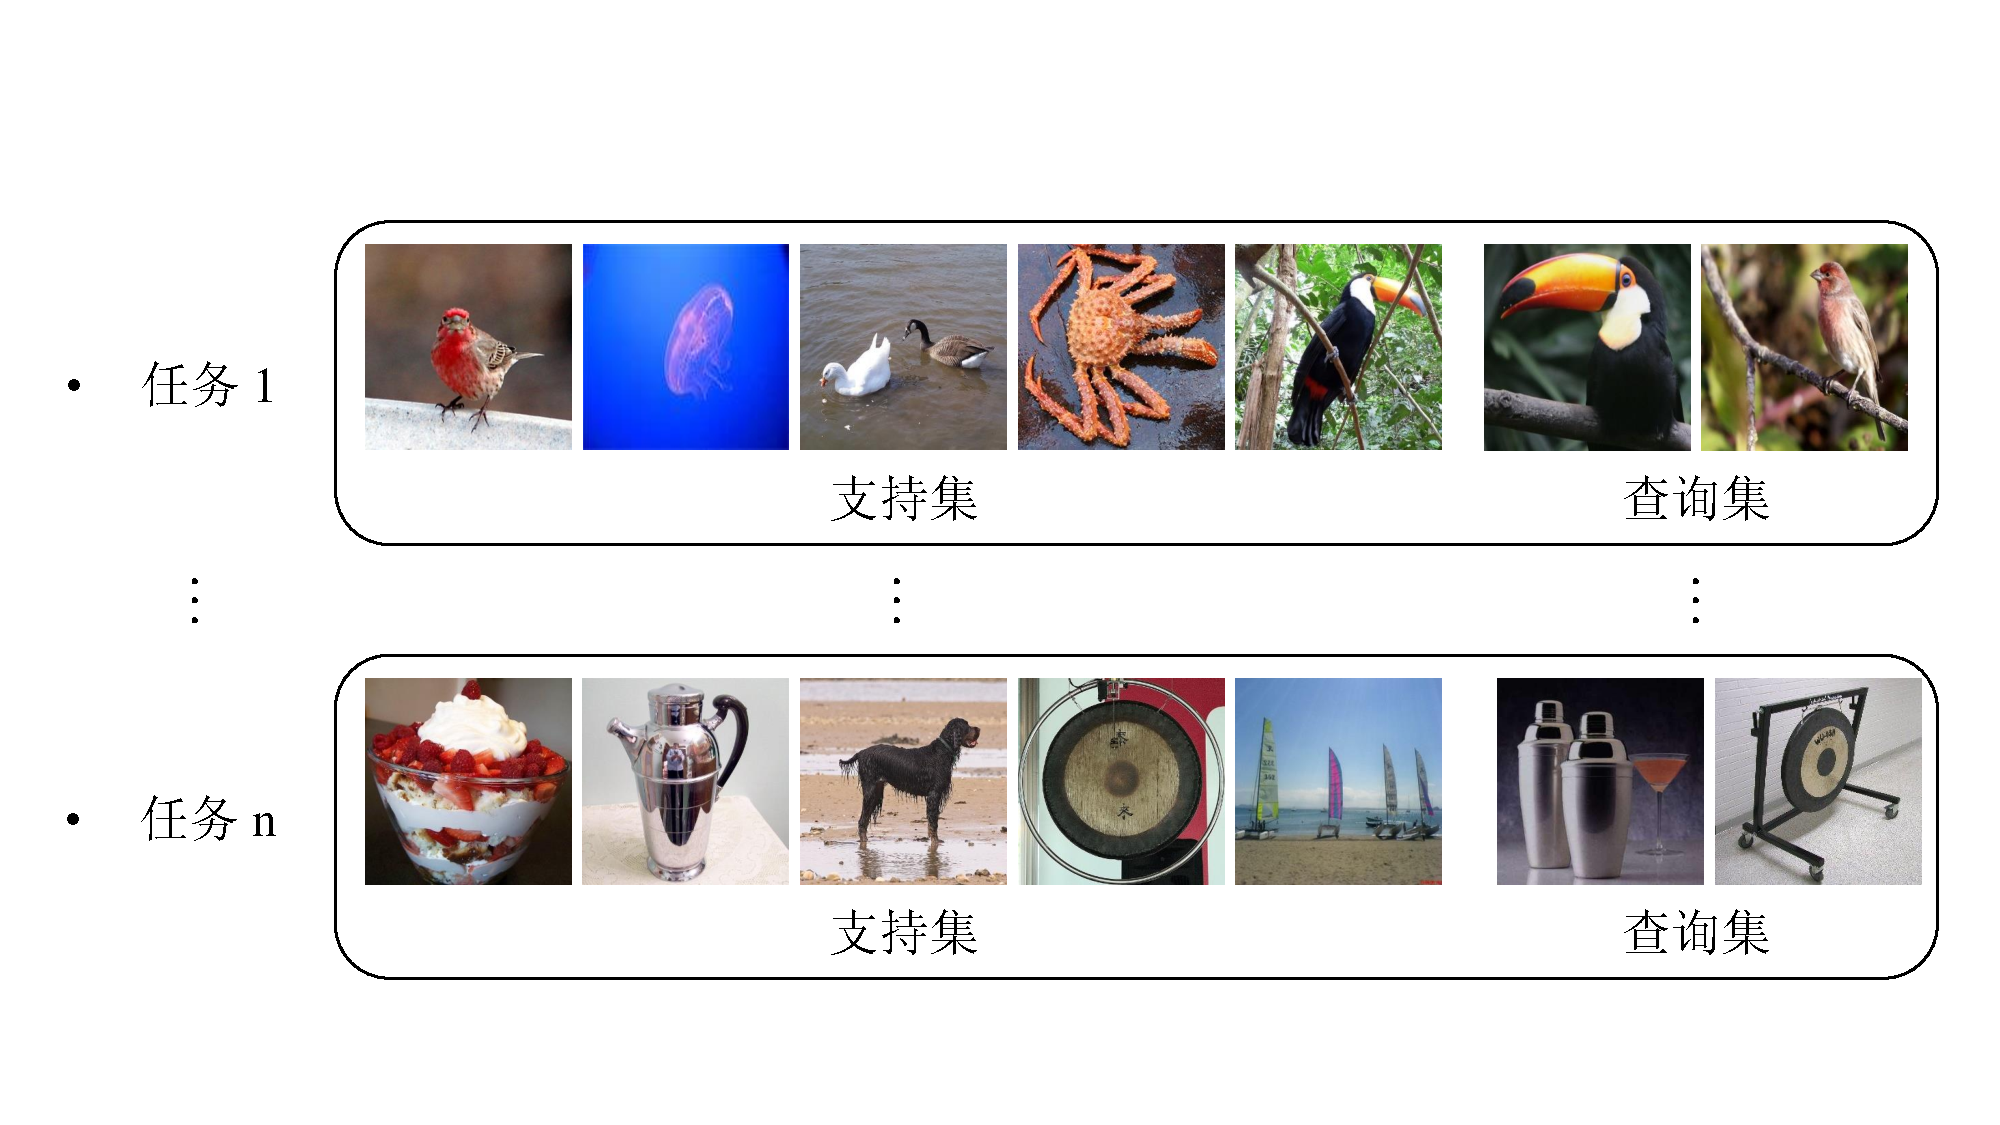
\includegraphics[width=1.0\columnwidth]{figures/RelatedWork/少样本分类测试任务.pdf}
\bicaption[少样本分类测试任务示意图]{少样本分类测试任务示意图。}[Illustration of few-shot classification testing tasks]{Illustration of few-shot classification testing tasks.}
\label{figure2: 少样本分类测试任务}
\end{figure}

\section[\hspace{-2pt}对比学习]{{\heiti\zihao{-3} \hspace{-8pt}对比学习}}\label{section2: 对比学习}

在计算机视觉领域,特征学习的方法越来越多样化。其中,对比学习以其独特的学习机制,即通过比较样本之间的相似性和差异性来提取鲜明且有区分度的特征表征,近年来受到了广泛的关注和研究。在图像处理任务中,对比学习已经证明了其在提高模型泛化能力和识别精度方面的显著效果,并被广泛应用到少样本分类问题中。根据对比学习是否使用数据集标签信息,可以将其分为无监督对比学习和有监督对比学习,以下将分别进行介绍。

\subsection[\hspace{-2pt}无监督对比学习]{{\heiti\zihao{4} \hspace{-8pt}无监督对比学习}}\label{section2: 无监督对比学习}

无监督对比学习不依赖于标注数据,它通常采用正负样本对的形式来构建训练任务。正样本对通常来自于同一实例的不同视角(例如,同一图像的不同数据增强版本),而负样本对则来自于不同实例。模型的目标是使得正样本对在表示空间中彼此接近,而负样本对彼此远离。该过程一般通过最小化InfoNCE损失函数实现,该损失函数如下式所示,
\begin{equation}
\label{equation2: infoNCE}
\mathcal{L} = - \text{log}\frac{\text{exp}(cos(f(x), f(x^+)) / \tau)}{\text{exp}(cos(f(x), f(x^+)) + \sum_{j=1}^{N} \text{exp}(cos(f(x), f(x^-))}.
\end{equation}
其中,图像$x$经由网络$f(\cdot)$后映射到特征空间,$x^+$,$x^-$分别代表$x$的正样本以及负样本,$N$为负样本数量。$cos(\cdot)$是余弦相似度,$\text{exp}(\cdot)$为以e为底的指数函数。

Chen等人\cite{SimCLR}提出了一个简单有效的无监督对比学习框架-SimCLR,旨在通过比较不同视角下图像的特征表示来学习强大的特征提取网络。SimCLR的核心思想是利用数据增强来产生正样本对,即从同一张图像中通过随机的数据增强操作(如裁剪、颜色变换等)生成两个视角,然后使来自同一图像的特征相互靠近,同时使得来自不同图像的特征尽可能地远离。尽管SimCLR在无监督特征学习方面取得了显著的成果,但其有一个明显缺点,即SimCLR的效果很大程度上依赖于对比损失函数中大量不同的负样本对,为了达到最佳性能,需要批次大小很大,这对计算资源的要求较高。He等人\cite{MoCo}提出的MoCo算法通过引入一个动态字典来存储样本特征表示解决了此问题。这个字典是一个队列,新的样本特征进入队列时,旧的样本特征被移除,以保持队列的固定大小。MoCo可通过此字典高效地采样大量负样本,因此不再需要使用很大的批次便可达到最佳效果。这些无监督对比学习方法特别适合于数据量大但未标注的场景,能够有效地利用大量未标注数据来学习有意义的特征表示。

% 通过无监督对比学习,模型能够捕捉到数据的内在结构和丰富的特征信息,这为后续的监督学习任务,如分类、检测等,提供了强大的预训练模型。此外,该方法也在自然语言处理、图数据分析等领域展现出了广泛的应用潜力。

\subsection[\hspace{-2pt}有监督对比学习]{{\heiti\zihao{4} \hspace{-8pt}有监督对比学习}}\label{section2: 有监督对比学习}

虽然无监督对比学习为使用大量无标注数据训练一个好的预训练模型提供了有效途径,但因为其在样本建模过程中将样本$x$与其负样本距离推远,而负样本中可能包含$x$的同类样本,这可能会学习到错误的样本关系。因此,Khosla等人\cite{SupCon}提出了有监督对比学习(Supervised Contrastive Learning,简称SupCon)对这个问题进行解决。SupCon是对比学习的一种变体,它结合了监督信号来进一步提升学习效率和特征表示的质量。与无监督对比学习相比,有监督对比学习在构造正负样本对时利用了标签信息,以确保模型不仅学会区分不同的样本,而且能够区分不同的类别,如图\ref{figure2: 对比学习}所示(此图来源于SupCon\cite{SupCon})。SupCon不仅保留了无监督对比学习中正样本对的概念,更进一步地,将属于同一类别的不同样本也视为正样本对,负样本对则是来自不同类别的样本,以此强化模型对不同类别间差异的识别能力。这种方法有效地缩小了同类样本间的表征距离,同时增强了不同类别间表征的区分度,有助于提升模型在复杂视觉任务中的表现。

\begin{figure}[h!]
\centering
\captionsetup{font={small, stretch=1.312}}
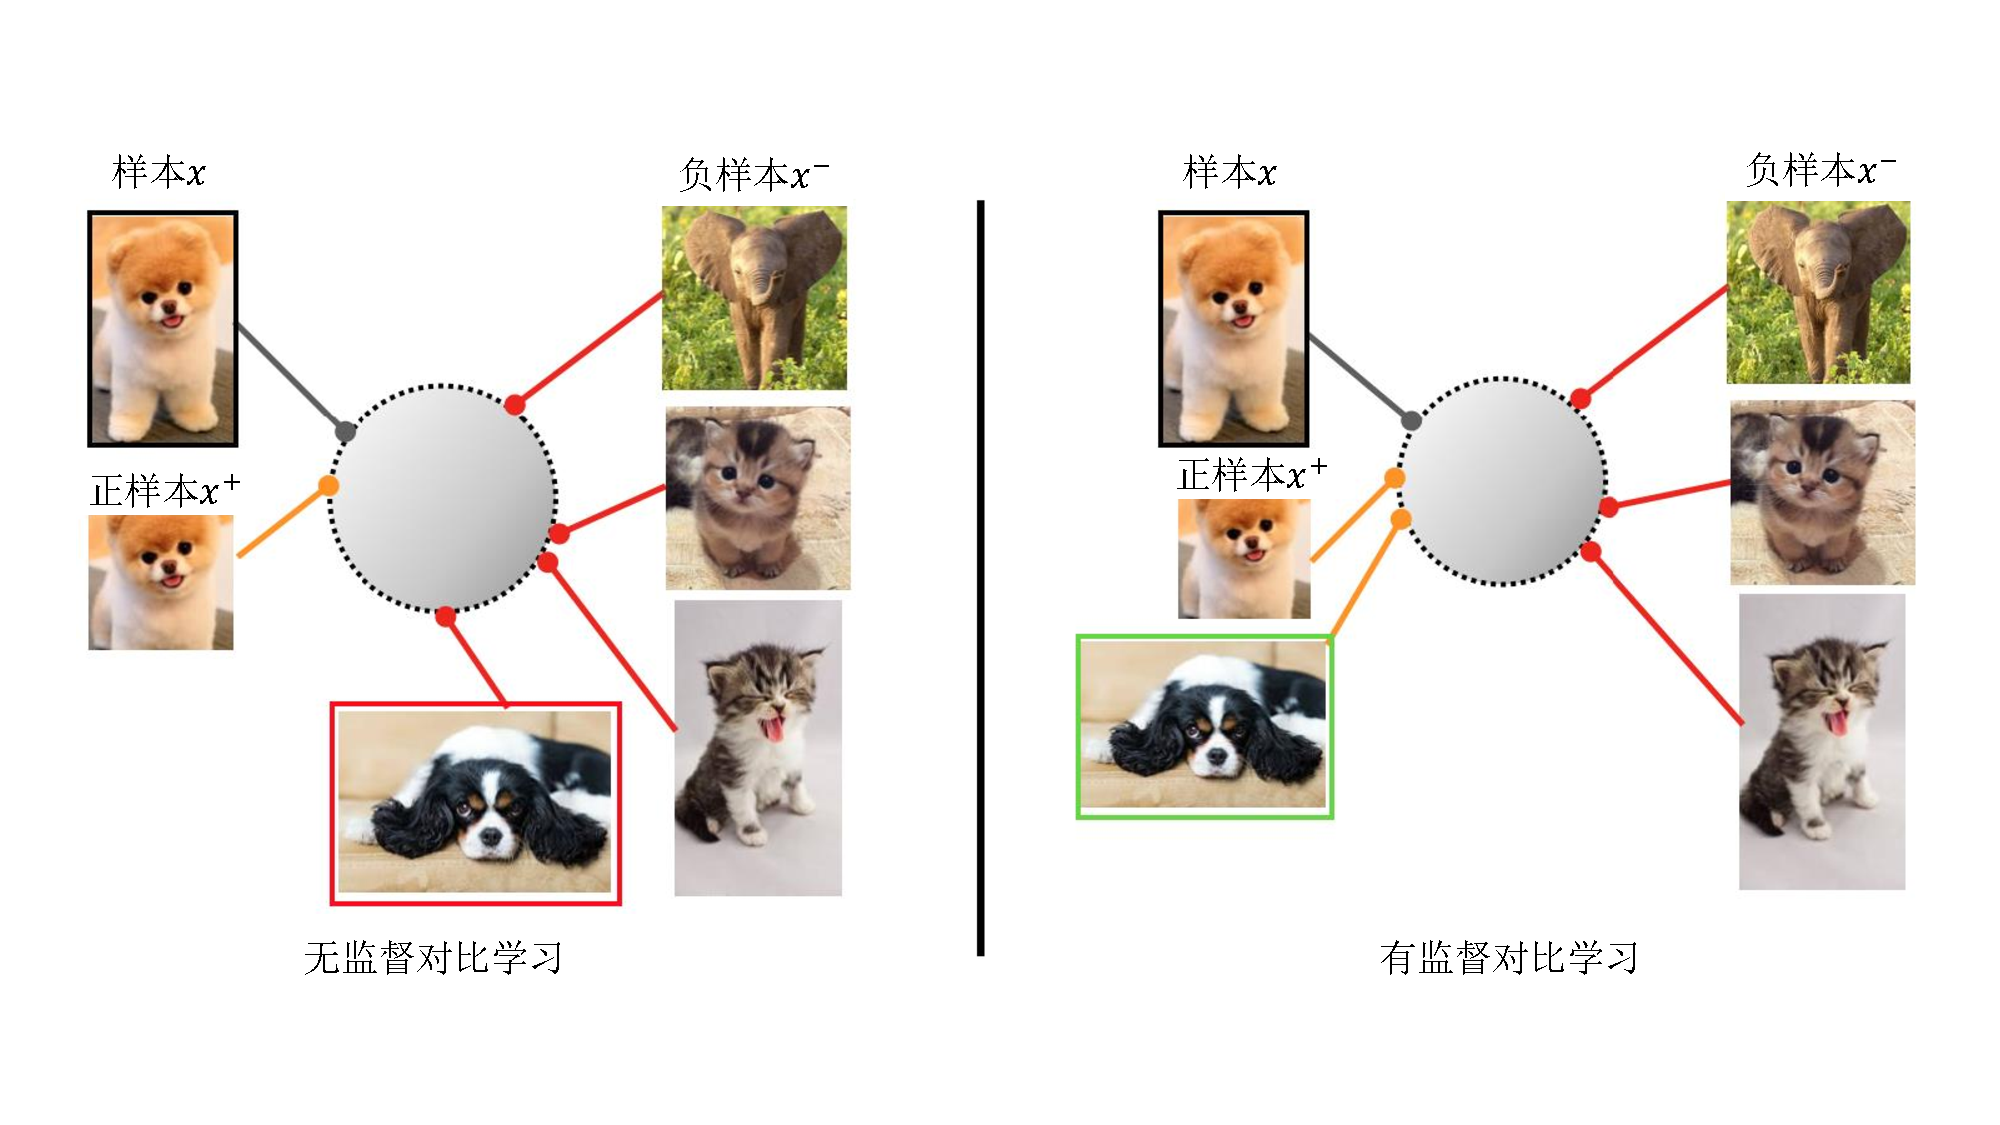
\includegraphics[width=1.0\columnwidth]{figures/RelatedWork/对比学习.pdf}
\bicaption[无监督对比学习与有监督对比学习]{无监督对比学习与有监督对比学习。}[Unsupervised Contrastive Learning VS Supervised Contrastive Learning]{Unsupervised Contrastive Learning VS Supervised Contrastive Learning.}
\label{figure2: 对比学习}
\end{figure}

\section[\hspace{-2pt}语义信息表示]{{\heiti\zihao{-3} \hspace{-8pt}语义信息表示}}\label{section2: 语义信息表示}

目前,在少样本分类问题中,很多工作开始使用语义信息以对视觉信息进行补充,使用的语义信息一般为用自然语言处理(Natural Language Processing,简称NLP)模型或多模态模型的文本编码器提取的语义特征。提取语义特征时,会将类别名称或提示文本与类别名称进行拼接之后的文本输入文本编码器,然后得到编码器输出的语义向量作为语义特征。以下对少样本分类中经常使用的语义特征提取模型进行介绍。

\subsection[\hspace{-2pt}Word2Vec]{{\heiti\zihao{4} \hspace{-8pt}Word2Vec}}\label{section2: Word2Vec}

Mikolov等人\cite{mikolov2013efficient, Word2Vec}提出的Word2Vec是一种广泛使用的自然语言处理技术,它从大量文本语料中以无监督的方式学习语义知识,旨在将词汇映射到稠密向量空间中,其中语义相似的词汇会在向量空间中彼此接近。Word2Vec包含两种训练模型:连续词袋(Continuous Bag-of-Words,简称CBOW)模型和跳跃(Continuous Skip-gram,简称Skip-Gram)模型,如图\ref{figure2: Word2Vec}所示(此图来源于Word2Vec\cite{Word2Vec})。

\textbf{CBOW模型:}CBOW模型通过上下文(周围的词汇)来预测当前词,如图\ref{figure2: Word2Vec}(左)所示。具体来说,它将上下文中的多个词汇作为输入,并尝试预测在这些上下文词汇中间的目标词汇。这个模型特别适合处理较小的数据集。

\textbf{Skip-Gram模型:}与CBOW相反,Skip-Gram模型使用一个词来预测其周围的上下文,如图\ref{figure2: Word2Vec}(右)所示。给定一个特定的词,目标是预测在一个特定范围内的前后词汇。Skip-Gram模型在处理大数据集时表现更好,尤其是对罕见词汇的表示更为有效。

\begin{figure}[h!]
\centering
\captionsetup{font={small, stretch=1.312}}
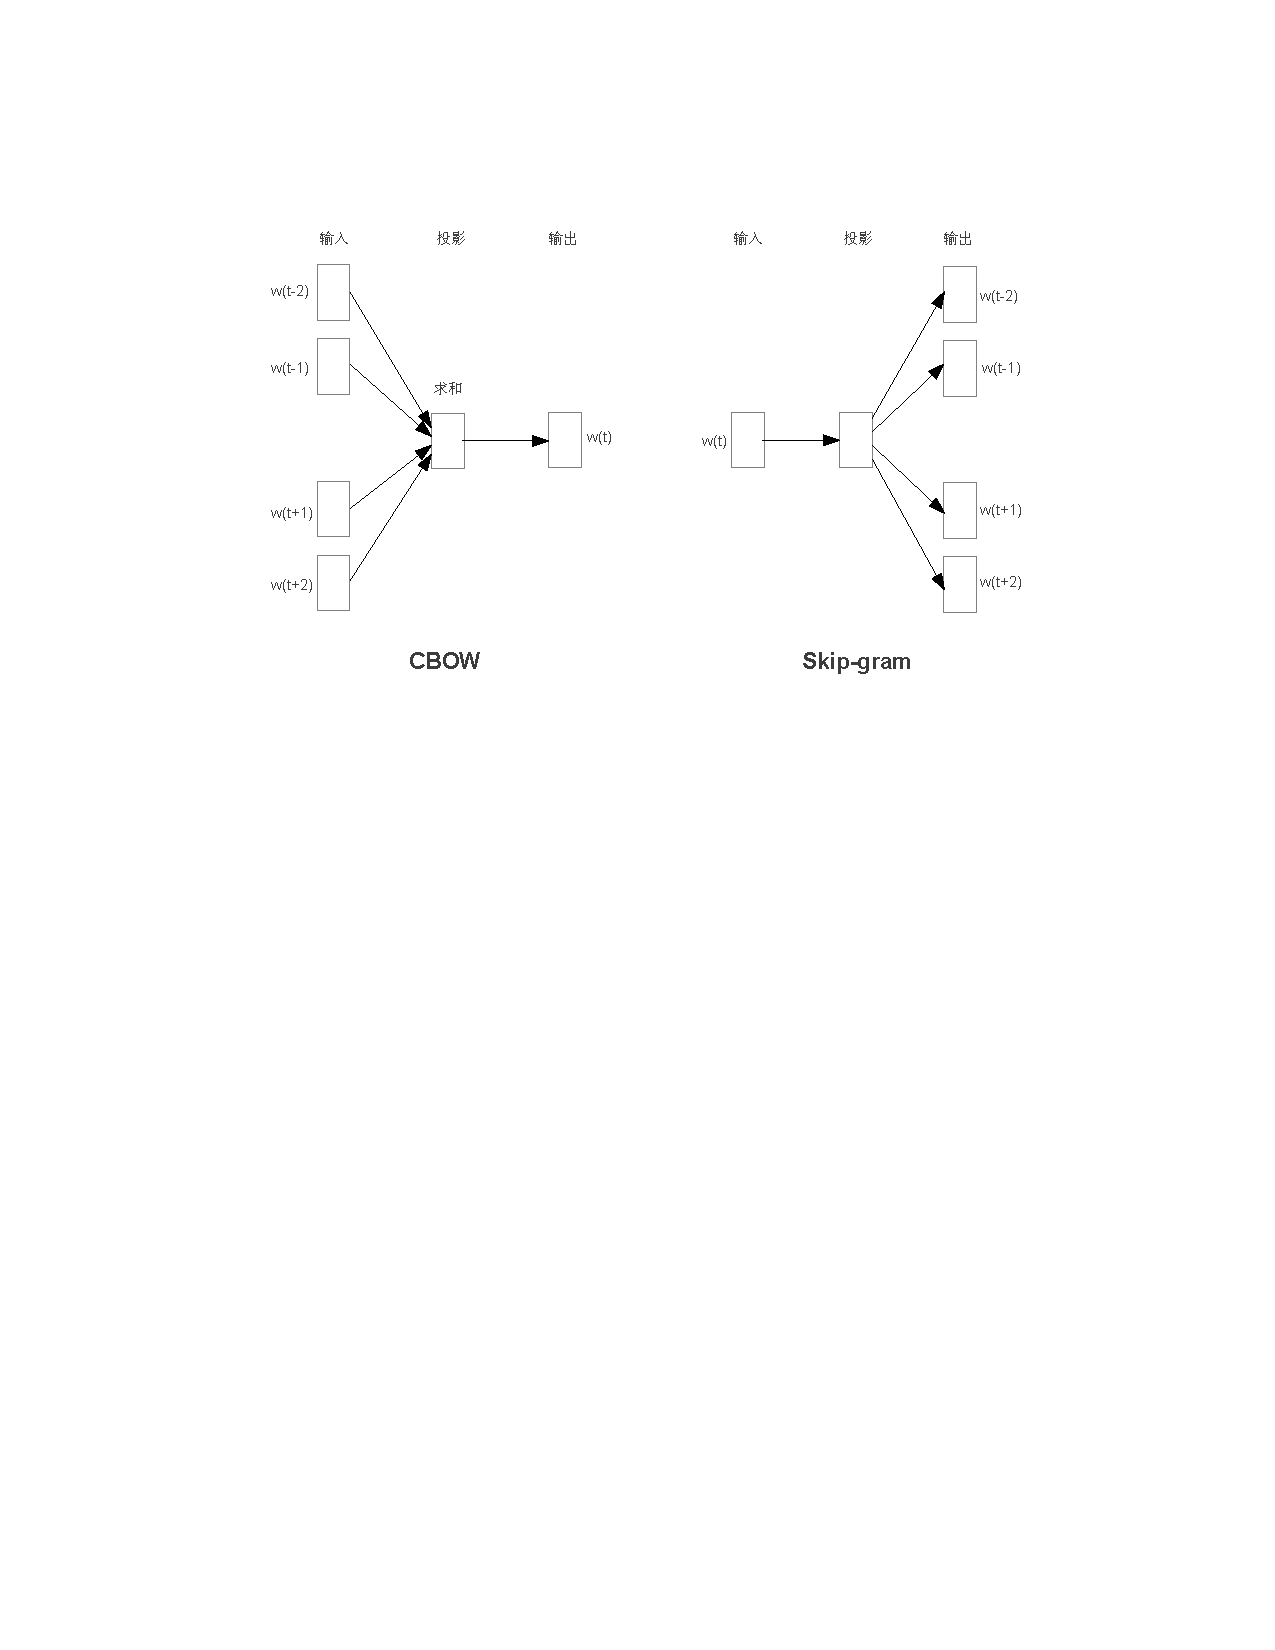
\includegraphics[width=1.0\columnwidth]{figures/RelatedWork/Word2Vec.pdf}
\bicaption[CBOW模型与Skip-Gram模型示意图]{CBOW模型与Skip-Gram模型示意图。}[Illustration of CBOW model and Skip-Gram model]{Illustration of CBOW model and Skip-Gram model.}
\label{figure2: Word2Vec}
\end{figure}

Word2Vec的核心优势在于它能够捕捉到词汇之间的细微语义关系,并通过向量运算来揭示词汇之间的语义相似性。这使得Word2Vec在诸多自然语言处理任务中得到广泛应用,包括文本相似性度量、情感分析、机器翻译以及作为深度学习模型的预训练层等,另外,很多计算机视觉任务也使用Word2Vec来提取语义特征以对视觉特征进行修正或补充。

\subsection[\hspace{-2pt}GloVe]{{\heiti\zihao{4} \hspace{-8pt}GloVe}}\label{section2: GloVe}

Pennington等人\cite{GloVe}提出的GloVe(Global Vectors for Word Representation)也是一种用于词嵌入的无监督学习算法。该模型旨在将单词映射到一个向量空间中,使得这些向量能够捕捉到词与词之间的共现关系,从而反映出词义的复杂模式和结构。GloVe模型的关键创新在于它结合了两种主流的词表示方法的优点:基于全局矩阵分解(Global Matrix Factorization)的方法和基于局部上下文窗口(Local Context Window)的方法。

GloVe的核心思想是首先构建一个全局词共现矩阵,记录整个语料库中各个词之间的共现次数,然后通过优化一个目标函数来学习词向量。这个目标函数旨在让共现次数的对数值与相应词向量的点积尽可能接近,同时引入偏置项来进一步提升模型的灵活性和准确性。具体来说,GloVe构建一个大型的词-词共现矩阵,矩阵中的每个元素代表了两个词在一定窗口大小内共同出现的次数。这一步捕获了全局的共现统计信息。然后其定义了一个特殊的损失函数,该损失函数不仅关注词对之间的共现概率,而且关注共现概率的比例,这有助于捕获词义之间更细微的差别。这个损失函数同时考虑到了共现次数的稀疏性和不均匀性。通过最小化损失函数,模型学习到的词向量能够反映出词与词之间的共现概率,这意味着词向量空间中的距离可以表示词义之间的相似度。这一步既利用了局部信息(通过具体的共现频率),也综合了全局信息(通过整个语料库的统计数据)。

\begin{figure}[h!]
\centering
\captionsetup{font={small, stretch=1.312}}
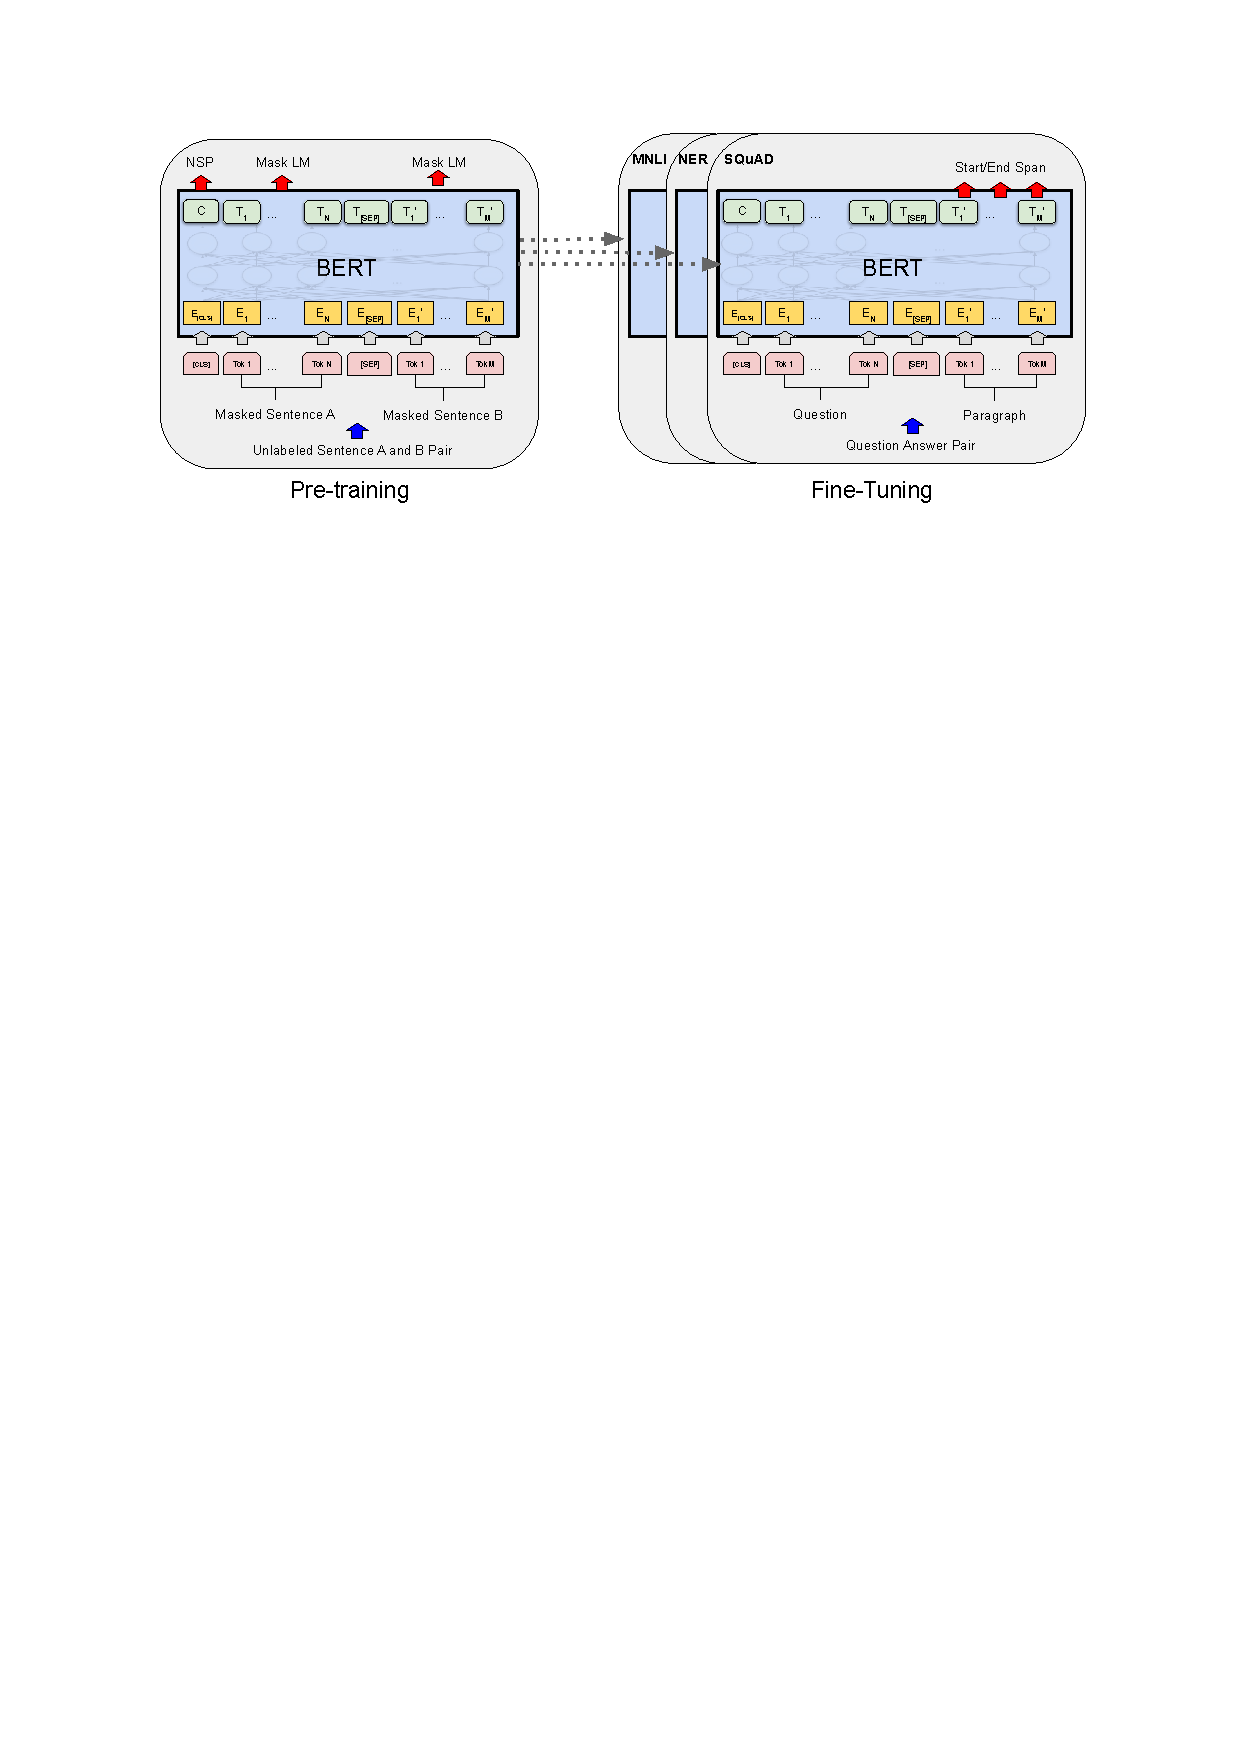
\includegraphics[width=1.0\columnwidth]{figures/RelatedWork/BERT.pdf}
\bicaption[BERT的整体预训练和微调过程]{BERT的整体预训练和微调过程。}[Overall pre-training and fine-tuning procedures for BERT]{Overall pre-training and fine-tuning procedures for BERT.}
\label{figure2: BERT}
\end{figure}

\subsection[\hspace{-2pt}BERT]{{\heiti\zihao{4} \hspace{-8pt}BERT}}\label{section2: BERT}

Devlin等人\cite{Bert}提出的BERT(Bidirectional Encoder Representations from Transformers)模型是一种革命性的自然语言处理模型。该模型利用了Transformer架构的双向编码器,能够理解语言的深层语义和上下文关系。BERT的创新之处在于其基于Transformer模型的编码器,使得它能够同时考虑词语左侧和右侧的上下文信息,这与以往的单向模型或浅层双向模型不同,使其能够更准确地理解词义。如图\ref{figure2: BERT}所示(此图来源于BERT\cite{Bert}),BERT模型首先在大规模的文本语料库上进行预训练,学习通用的语义表示,然后针对具体的NLP任务进行微调,这一过程极大提升了模型在特定任务上的性能。由于其良好的性能与开创性,后续又出现了诸如SBERT\cite{SBERT}、RoBERTa\cite{RoBERTa}、ALBERT\cite{ALBERT}等改进工作。BERT模型通过两种类型的预训练任务学习语义表示:

\noindent \textbf{(1)掩码语言模型(Masked Language Model,简称MLM):}在训练过程中,BERT会随机遮蔽模型输入句子中的一部分词语(使用[MASK] token代替原有输入),然后让模型预测这些遮蔽的词语,这可以迫使模型学习到词语的双向上下文关系。另外,为了解决模型微调期间从未看到[MASK] token的问题,BERT模型不总是直接用[MASK] token代替所选单词,而是将所选单词80\%的概率替换为[MASK] token,10\%的概率用一个随即单词替换所选单词,剩下10\%的概率则是保持其不变。

\noindent \textbf{(2)下一句预测(Next Sentence Prediction,简称NSP):}由于很多NLP下游任务都是基于理解两个句子之间的关系,如问答和自然语言推断,因此BERT设计了一个下一句预测的任务。给定两个句子A和B,模型需要预测B是否是A的下一句,这可以帮助模型理解句子间的关系。

\begin{figure}[h!]
\centering
\captionsetup{font={small, stretch=1.312}}
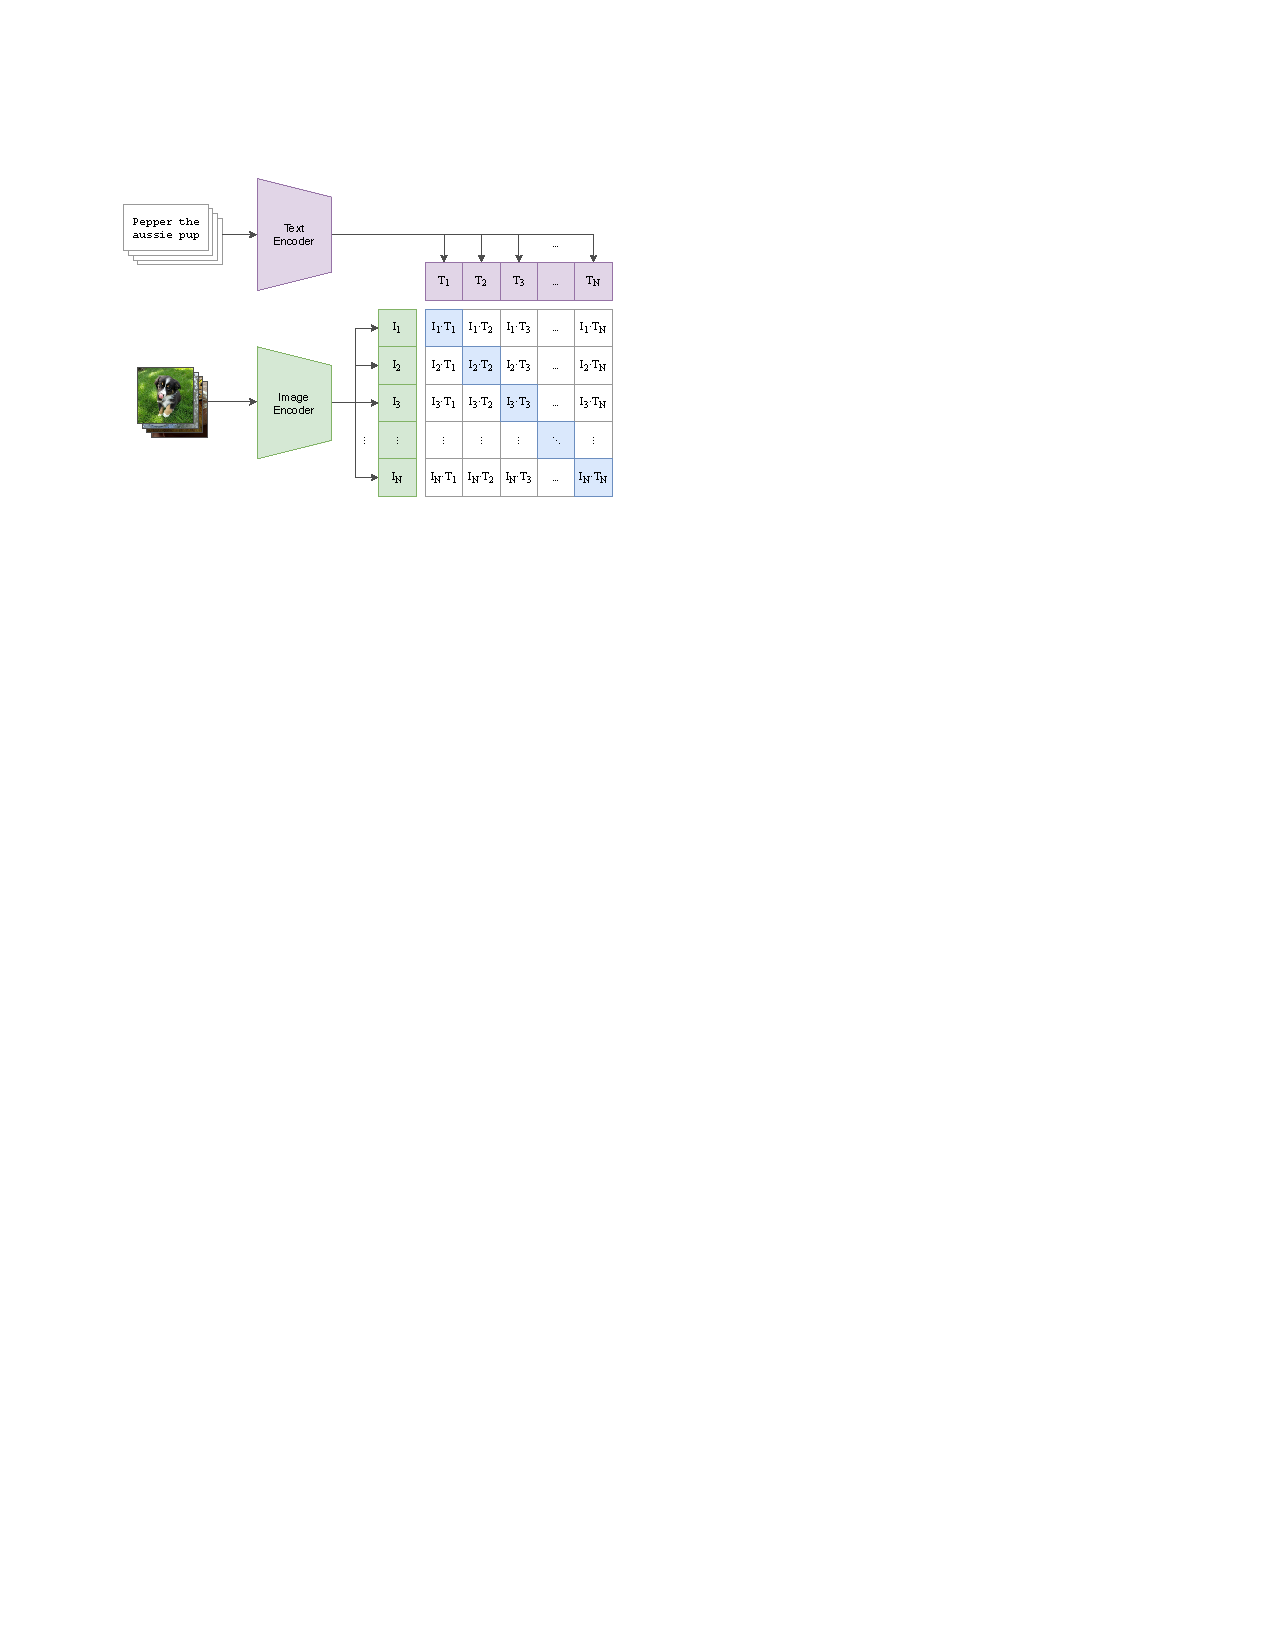
\includegraphics[width=0.8\columnwidth]{figures/RelatedWork/CLIP.pdf}
\bicaption[CLIP模型预训练示意图]{CLIP模型预训练示意图。}[Illustration of pre-training CLIP model]{Illustration of pre-training CLIP model.}
\label{figure2: CLIP}
\end{figure}

\subsection[\hspace{-2pt}CLIP]{{\heiti\zihao{4} \hspace{-8pt}CLIP}}\label{section2: CLIP}

近年来,Radford等人\cite{Clip}提出的CLIP(Contrastive Language–Image Pre-training)模型受到了很多研究者的关注,并促进了多模态大模型和一些其他任务的发展。CLIP旨在通过大规模的图文对比学习来同时理解图像和文本,并建立它们之间的联系。CLIP模型的创新之处在于其跨模态能力,它不仅能理解图片内容,也能理解与图片内容相对应的文本描述,从而在多种视觉任务上展示出了卓越的性能和强大的泛化能力,并提供了一个充分建模文本关系的文本编码器。

如图\ref{figure2: CLIP}所示(此图来源于CLIP\cite{Clip}),CLIP由两部分组成:一个图像编码器和一个文本编码器。图像编码器负责提取图像的视觉特征,而文本编码器则提取文本的语义特征。这两个编码器可以是任何形式的神经网络。在原始CLIP模型中,图像编码器基于Vision Transformer(ViT)或ResNet架构,而文本编码器基于Transformer架构。CLIP的训练过程涉及大量图像和文本对的对比学习。具体来说,模型训练的目标是最大化相匹配的图像和文本对之间的相似度,同时最小化不匹配对的相似度。这种训练方式使得CLIP学习到的特征表示能够跨越视觉和语义的界限,理解两种模态之间的对应关系。

\section[\hspace{-2pt}数据集及评价指标]{{\heiti\zihao{-3} \hspace{-8pt}数据集及评价指标}}\label{section2: 数据集及评价指标}

本文使用四个少样本分类基准数据集对模型性能进行评估,包括三个普通少样本分类数据集:miniImageNet \cite{vinyals2016matching}、tieredImageNet \cite{ren2018meta}、CIFAR-FS \cite{bertinetto2018meta},以及一个细粒度数据集:CUB-200-2011(CUB)\cite{wah2011caltech},以下对其进行分别介绍,并对少样本分类评价指标进行描述。

\begin{table}[h!]
\small    % 设置表格字体为5号
\setstretch{1.245}        % 设置具有指定弹力的橡皮长度(原行宽的1.2倍)
\captionsetup{font={small, stretch=1.512}}
\centering
\bicaption[miniImageNet、CIFAR-FS和CUB的数据集划分]{miniImageNet、CIFAR-FS和CUB的数据集划分。}[Dataset partition of miniImageNet, CIFAR-FS and CUB]{Dataset partition of miniImageNet, CIFAR-FS and CUB.}    % 中英文标题
\begin{tabularx}{\textwidth}{lCCCC}
\toprule
\multirow{2}*{数据集} & \multicolumn{4}{c}{类别数目} \\
\cline{2-5}
& \raisebox{-2pt}{训练集} & \raisebox{-2pt}{验证集} & \raisebox{-2pt}{测试集} & \raisebox{-2pt}{总数} \\
\midrule
miniImageNet & 64 & 16 & 20 & 100 \\
CIFAR-FS & 64 & 16 & 20 & 100 \\
CUB & 100 & 50 & 50 & 200 \\
\bottomrule
\end{tabularx}
\vspace{-20pt}
\label{table2: dataset1}
\end{table}

\begin{table}[h!]
\small    % 设置表格字体为5号
\setstretch{1.245}        % 设置具有指定弹力的橡皮长度(原行宽的1.2倍)
\captionsetup{font={small, stretch=1.512}}
\centering
\bicaption[tieredImageNet的数据集划分]{tieredImageNet的数据集划分。}[Dataset partition of tieredImageNet]{Dataset partition of tieredImageNet.}    % 中英文标题
\begin{tabularx}{\textwidth}{XCCCC}
\toprule
\multirow{2}*{类别层级} & \multicolumn{4}{c}{类别数目} \\
\cline{2-5}
& \raisebox{-2pt}{训练集} & \raisebox{-2pt}{验证集} & \raisebox{-2pt}{测试集} & \raisebox{-2pt}{总数} \\
\midrule
超类 & 20 & 6 & 8 & 34 \\
子类 & 351 & 97 & 160 & 608 \\
\bottomrule
\end{tabularx}
\label{table2: dataset2}
\end{table}

\subsection[\hspace{-2pt}数据集]{{\heiti\zihao{4} \hspace{-8pt}数据集}}\label{section2: 数据集}

miniImageNet数据集\cite{vinyals2016matching}和tieredImageNet数据集\cite{ren2018meta}均为ImageNet\cite{deng2009imagenet}的子集。其中,miniImageNet数据集包含100个类别,每个类别有600张图像。本文遵循Ravi等人\cite{optimization}提出的划分准则,训练集、验证集和测试集分别包含64、16和20个类别。tieredImageNet数据集则包含34个超类(608个子类),分为20个训练类别(351个子类)、6个验证类别(97个子类)和8个测试类别(160个子类)。CIFAR-FS数据集\cite{bertinetto2018meta}源自CIFAR-100数据集,该数据集包含64个训练类别、16个验证类别和20个测试类别,每个类别同样有600张图像。Caltech-UCSD Birds(CUB)-200-2011(简称CUB)数据集\cite{wah2011caltech}则是一个包含不同种类的鸟类细粒度图像数据集,包含11788个图像样本,分为200个类别。根据Triantafillou等人\cite{triantafillou2017few}的划分准则,该数据集包含100个训练类别、50个验证类别和50个测试类别。各数据集划分如表\ref{table2: dataset1}和\ref{table2: dataset2}所示。

\subsection[\hspace{-2pt}评价指标]{{\heiti\zihao{4} \hspace{-8pt}评价指标}}\label{section2: 评价指标}

对于所有数据集,本文评估5-way 1-shot 以及5-way 5-shot少样本分类任务性能。在一次模型评估中,本文方法采样2000个少样本分类任务,并计算了95\%置信区间的平均分类准确率作为模型的评价指标。在一个少样本分类任务中,每个类别的支持集样本数目为1或5(根据任务决定),查询集样本数目为15,与其他方法\cite{RFS, IER}保持一致。

\section[\hspace{-2pt}本章小结]{{\heiti\zihao{-3} \hspace{-8pt}本章小结}}\label{section2: 本章小结}

本章首先详细介绍了少样本分类任务的定义及其训练测试过程。然后对后续研究工作所涉及到的相关技术进行了介绍,其中包括第三章所使用到的对比学习技术,根据是否使用数据集标签信息将其分为无监督对比学习和有监督对比学习进行了详细阐述;以及第四章所使用到的语义信息表示,介绍了如何提取语义信息表示和少样本分类中常用的语义特征提取模型。最后,介绍了本文方法所使用到的少样本分类数据集和评价指标。
